%%%%%%%%%%%%%%%%%%%%%%%%%%%%%%%%%%%%%%%%%
% Beamer Presentation
% LaTeX Template
% Version 1.0 (10/11/12)
%
% This template has been downloaded from:
% http://www.LaTeXTemplates.com
%
% License:
% CC BY-NC-SA 3.0 (http://creativecommons.org/licenses/by-nc-sa/3.0/)
%
%%%%%%%%%%%%%%%%%%%%%%%%%%%%%%%%%%%%%%%%%

%----------------------------------------------------------------------------------------
%	PACKAGES AND THEMES
%----------------------------------------------------------------------------------------

\documentclass{beamer}

\mode<presentation> {

% The Beamer class comes with a number of default slide themes
% which change the colors and layouts of slides. Below this is a list
% of all the themes, uncomment each in turn to see what they look like.

%\usetheme{default}
%\usetheme{AnnArbor}
%\usetheme{Antibes}
%\usetheme{Bergen}
%\usetheme{Berkeley}
%\usetheme{Berlin}
%\usetheme{Boadilla}
%\usetheme{CambridgeUS}
%\usetheme{Copenhagen}
%\usetheme{Darmstadt}
%\usetheme{Dresden}
%\usetheme{Frankfurt}
%\usetheme{Goettingen}
%\usetheme{Hannover}
%\usetheme{Ilmenau}
%\usetheme{JuanLesPins}
%\usetheme{Luebeck}
\usetheme{Madrid}
%\usetheme{Malmoe}
%\usetheme{Marburg}
%\usetheme{Montpellier}
%\usetheme{PaloAlto}
%\usetheme{Pittsburgh}
%\usetheme{Rochester}
%\usetheme{Singapore}
%\usetheme{Szeged}
%\usetheme{Warsaw}

% As well as themes, the Beamer class has a number of color themes
% for any slide theme. Uncomment each of these in turn to see how it
% changes the colors of your current slide theme.

%\usecolortheme{albatross}
%\usecolortheme{beaver}
%\usecolortheme{beetle}
%\usecolortheme{crane}
%\usecolortheme{dolphin}
%\usecolortheme{dove}
%\usecolortheme{fly}
%\usecolortheme{lily}
%\usecolortheme{orchid}
%\usecolortheme{rose}
%\usecolortheme{seagull}
%\usecolortheme{seahorse}
%\usecolortheme{whale}
%\usecolortheme{wolverine}

%\setbeamertemplate{footline} % To remove the footer line in all slides uncomment this line
%\setbeamertemplate{footline}[page number] % To replace the footer line in all slides with a simple slide count uncomment this line

%\setbeamertemplate{navigation symbols}{} % To remove the navigation symbols from the bottom of all slides uncomment this line
}

\usepackage{graphicx} % Allows including images
\usepackage{booktabs} % Allows the use of \toprule, \midrule and \bottomrule in tables
\usepackage{multirow}
%----------------------------------------------------------------------------------------
%	TITLE PAGE
%----------------------------------------------------------------------------------------


\title[Experimental Design Project]{Maximizing Image Diversity for fMRI studies}

\author{Charles Zheng} % Your name
\institute[Stanford] % Your institution as it will appear on the bottom of every slide, may be shorthand to save space
{Stanford University}
\date{\today} % Date, can be changed to a custom date

\begin{document}

\begin{frame}
\titlepage % Print the title page as the first slide
\end{frame}

\section{Introduction}

\begin{frame}
\frametitle{How should researchers choose images?}
\begin{itemize}
\item \emph{Relevance}. Using natural images, because we care about how the brain percieves typical scenes in the real world.
\item \emph{Control}. Using artificially generated images (like gratings) with known parameters
\item \emph{Diversity}. Using a broad set of images to convincingly demonstrate generalizability
\end{itemize}
In this work we only deal with the question of \emph{diversity}
\end{frame}

\begin{frame}
\frametitle{Questions about diversity}
\begin{enumerate}
\item How can we define diversity?
\item How can researchers maximize this measure of diversity in their image set?
\item How does diversity affect metrics such as classification performance?
\item How can diversity improve generalizability?
\end{enumerate}

To explore these questions, we use the dataset from \emph{Kay et al.}
\end{frame}

\section{Defining diversity}

\frame{\sectionpage}

\begin{frame}
\frametitle{Defining diversity}
\begin{itemize}
\item A first step in defining diversity is \emph{dimensionality reduction} of images to a low-dimensional representation
\item Next, we need a \emph{distance metric} on the low-dimensional space
\item With coordinates and a distance metric, we can define a measure of diversity
\end{itemize}
\end{frame}

\begin{frame}
\frametitle{Dimensionality reduction}
\begin{itemize}
\item Suppose we have ``training data'' for $K$ images
\item A $K \times p_f$ matrix $X$ of image features (e.g. Gabor filters)
\item A $K \times p_v$ matrix $Y$ of mean voxel responses
\item Use \emph{sparse canonical correlation analysis} to find a $p_f
  \times d$ image basis $U$ and a $p_v \times d$ voxel basis $V$
\item Use the image basis $U$ to define coordinates
\end{itemize}
\end{frame}

\begin{frame}
\frametitle{Data: $V$ (voxel) basis}
\begin{center}
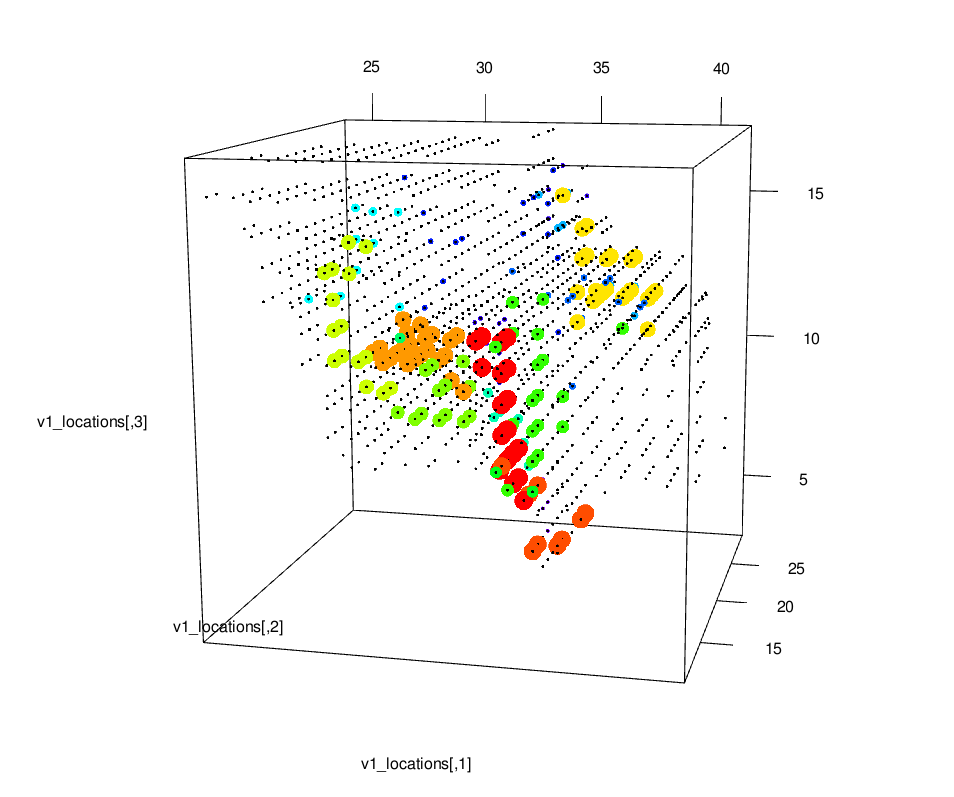
\includegraphics[scale=0.3]{cca1.png}
\end{center}
\end{frame}

\begin{frame}
\frametitle{Data: $V$ (voxel) basis}
\begin{center}
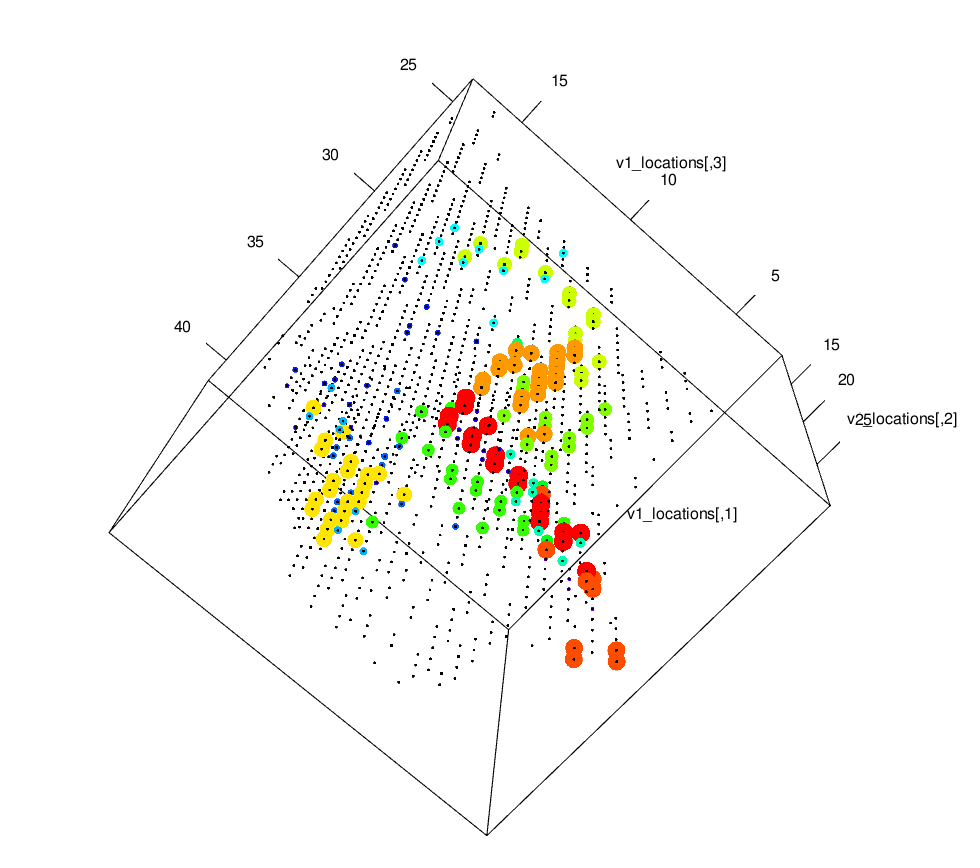
\includegraphics[scale=0.25]{cca2.png}
\end{center}
\end{frame}

\begin{frame}
\frametitle{Data: $U$ (image) basis}
\begin{center}
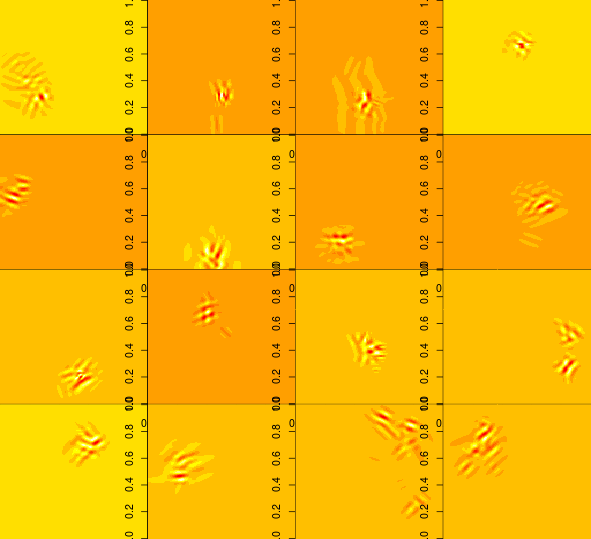
\includegraphics[scale=0.3]{cca3.png}
\end{center}
\end{frame}

\begin{frame}
\frametitle{A measure of diversity}
\begin{itemize}
\item We have coordinates $z$ for any image, and a distance metric $d(z_1, z_2)$
\item Suppose that the coordinates of all images form a connected, compact support set $S$
\item We will define the diversity of a distribution $P$ supported on $S$
\item Let $Z_1$, $Z_2$ be random points drawn from $P$
\item Let $\kappa(\cdot)$ be a bounded monotone decreasing function which goes to zero at infinity
\item Define the diversity of $P$ as
\[
-\mathbb{E}[\kappa(d(Z_1, Z_2))]
\]
\end{itemize}
\end{frame}

\begin{frame}
\frametitle{A measure of diversity}
\begin{itemize}
\item Let $\kappa(\cdot)$ be a bounded monotone decreasing function which goes to zero at infinity
\item Define the diversity of $P$ as
\[
-\mathbb{E}[\kappa(d(Z_1, Z_2))]
\]
\item We did not define the function $\kappa$... but in some sense the choice is unimportant!
\item Claim: let $h$ be a bandwidth, and let 
\[P_{\kappa, h} = \text{argmin} \mathbb{E}[k(d(Z_1, Z_2)/h)]\]
Then let $P_\kappa = \lim_{h \to 0} P_{\kappa, h}$.
There exist a unique distribution $U$ such that for all $\kappa$ satisfying a \emph{postive definite} condition, $P_\kappa = U$.
We call $U$ the \emph{uniform distribution}
\end{itemize}
\end{frame}

\begin{frame}
\frametitle{Example}
\begin{itemize}
\item Choose $\kappa(d) = \exp(-d^2)$, and various $h$
\item Let $d_{i,j}$ be the pairwise distances.
Measure the diversity of the image set by
\[
-\frac{1}{n^2} \sum_{i=1}^n \sum_{j = 1}^n \exp(-(d_{i,j}/h)^2)
\]
\item For $h=1$, diversity of the validation set (120 images) is -0.008,
diversity of the training set (1750 images) is -0.00057.
\item For $h=5$, diversity of the validation set (120 images) is -0.01,
diversity of the training set (1750 images) is -0.003.
\item The training set is more diverse
\end{itemize}
\end{frame}

\section{Maximizing diversity}

\frame{\sectionpage}

\begin{frame}
\frametitle{Choosing a diverse image set}
\begin{itemize}
\item Consider a database of $i = 1, \hdots, N$ images
\item Any selection of images is a uniform distribution on a subset of
$\{1, \hdots, N\}$ which can be represented by a vector $w$
\item Given a kernel $\kappa$ and bandwidth $h$, find the most diverse $w$ by
\[
\min_w w^T K w \text{ st }w \geq 0, ||w||_1 = 1
\]
where $K$ has entries $k_{ij} = \kappa(d_{ij}/h)$.
\item Finding the \emph{optimal} weight vector $w$ of a given sparsity
  is NP-hard.
However by increasing the bandwidth $h$ we naturally get sparse solutions.
\end{itemize}
\end{frame}

\begin{frame}
\frametitle{Optimal $w$ in 120 validation images}
\begin{tabular}{ccc}
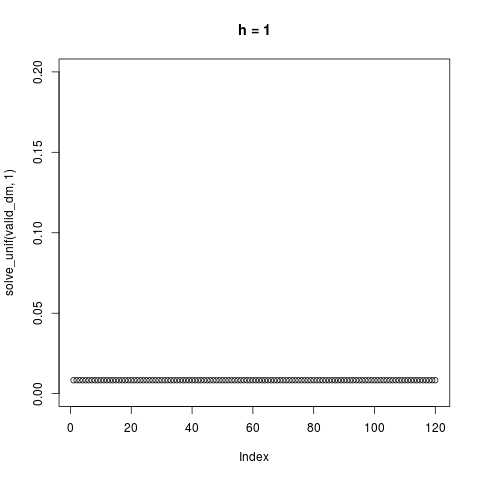
\includegraphics[scale=0.2]{valid_weight1.png} &
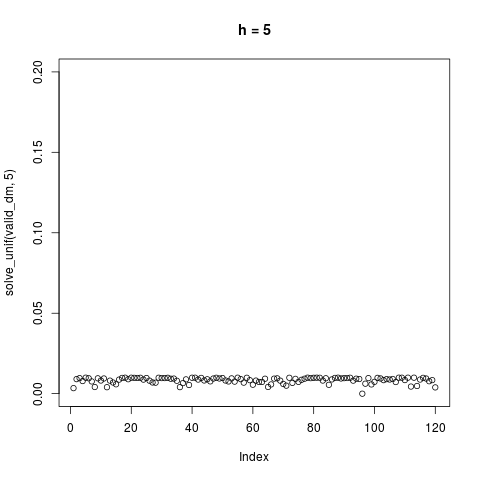
\includegraphics[scale=0.2]{valid_weight5.png} &
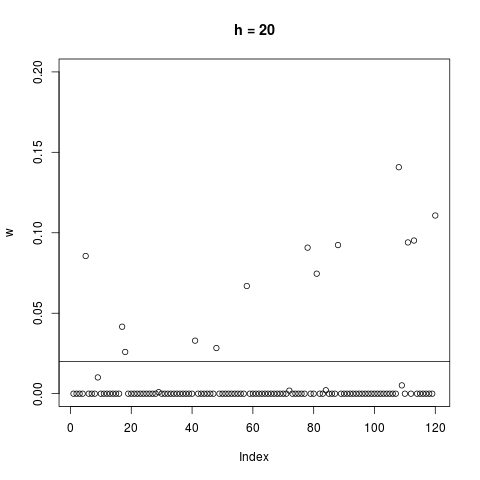
\includegraphics[scale=0.2]{valid_weight20.png}
\end{tabular}
\begin{center}
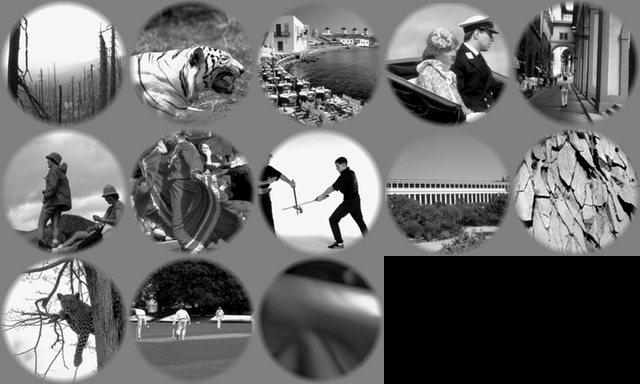
\includegraphics[scale=0.3]{valid_20.png}
\end{center}
\end{frame}

\section{Effect of diversity on misclassification}

\frame{\sectionpage}

\begin{frame}
\frametitle{Misclassification rates from Kay et al}
\begin{center}
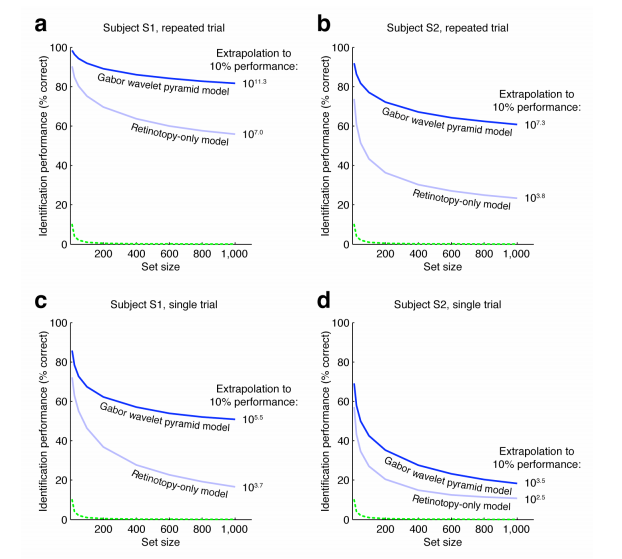
\includegraphics[scale=0.3]{kay_screenshot.png}
\end{center}
\end{frame}

\begin{frame}
\frametitle{Setup for misclassification rates}
\begin{itemize}
\item Fix a number $n$ of images
\item Pick $n$ images at random \emph{with replacement} from the
  database of $N$ images
\item (Sampling with replacement discourages deliberately using a
  small image database)
\item Assess misclassification rate of images from fMRI data using
  whatever method (encoding/decoding method, or standard
  classification)
\end{itemize}
\end{frame}

\begin{frame}
\frametitle{Distribution for the images?}
\begin{itemize}
\item Standard approach: pick $n$ images uniformly from database
\item What if your database has an unusually high proportion of a
  certain kind of image?
\item Alternative proposal: pick $n$ images with \emph{probability
  weighted} by an arbitrary $w$
\item Result: researchers would be incentivized to choose optimally
  uniform $w$.
\end{itemize}
\end{frame}

\begin{frame}
\frametitle{Theoretical model}
A theoretical model for misclassification with random images:
\begin{itemize}
\item Let $P$ be a distribution with support $S$, with density $p(x)$
\item Generate $n$ random images: their mean fMRI responses are
  $\mu_1, \hdots, \mu_n \sim P$
\item The observed fMRI responses for the $i$th image are $y_i^1,\hdots, y_i^{m_i} \sim N(\mu_i, \sigma^2 I)$
\end{itemize}
\end{frame}

\begin{frame}
\frametitle{Theoretical model}
\begin{center}
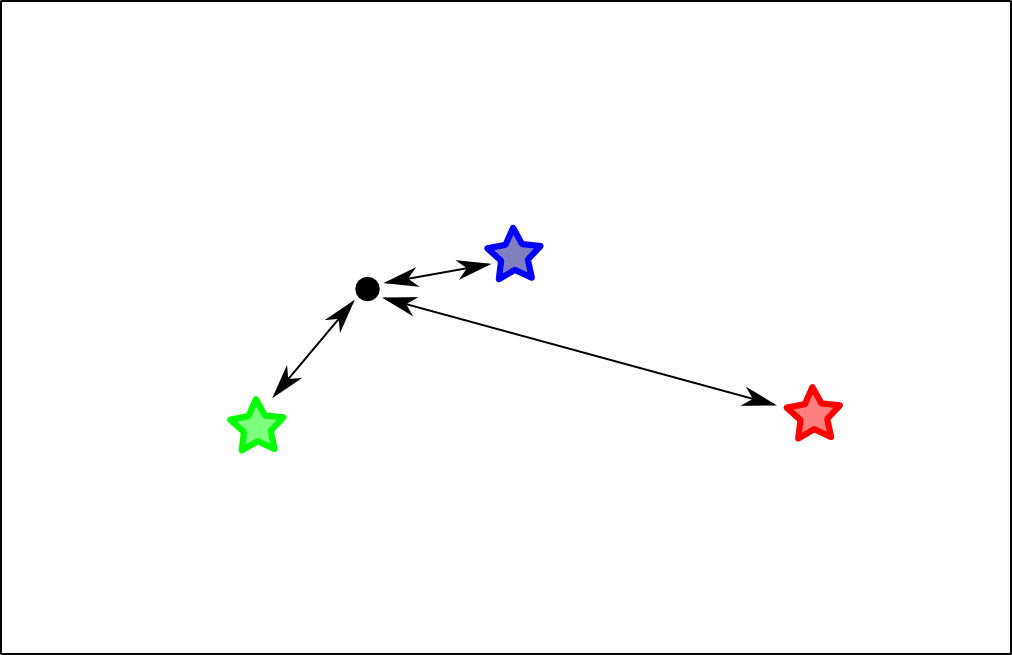
\includegraphics[scale=0.5]{fig02.png}
\end{center}

Suppose further that the true $\mu_i$ are known.
Then, points are classified based on nearest $\mu_i$.
\end{frame}

\begin{frame}
\frametitle{Theoretical model}
\begin{center}
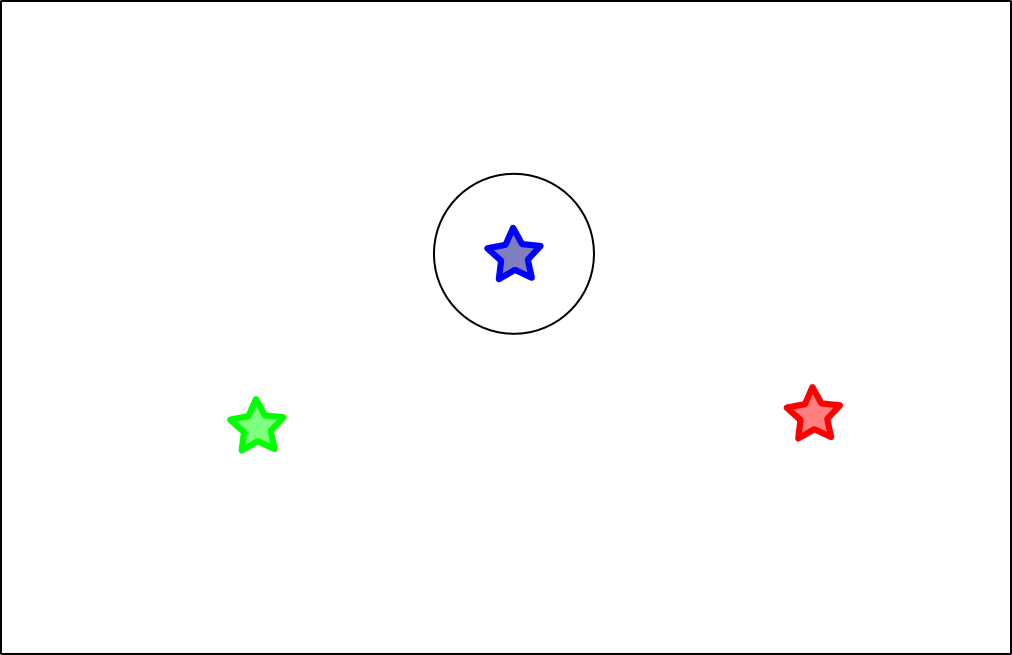
\includegraphics[scale=0.5]{fig03.png}
\end{center}

In a high dimension $d$, the distance of $y_i^\ell$ from $\mu_i$ approaches a
constant, $r_d$ due to \emph{concentration of measure}.
\end{frame}

\begin{frame}
\frametitle{Theoretical model}
\begin{center}
\begin{tabular}{ccc}
Correct! & & Incorrect...\\
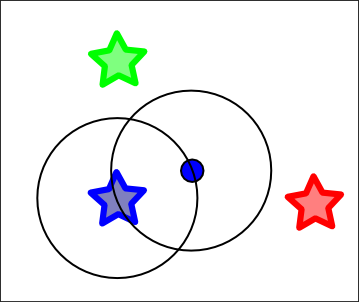
\includegraphics[scale=0.5]{fig04a.png} & & 
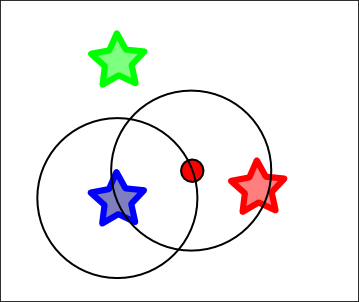
\includegraphics[scale=0.5]{fig04b.png}
\end{tabular}
\end{center}

Whether a given point $y_i^\ell$ is classified correctly depends on
whether or not there exist any other $\mu_j$ within radius $r_d$ of
$y_i^\ell$.
\end{frame}



\begin{frame}
\frametitle{Theoretical model}
\begin{itemize}
\item An exact expression for average misclassification rate is
\[
1 - \int_S \underbrace{p(\mu)}_{\text{distribution of }\mu}
\left[
\int_S \underbrace{\phi((\mu - y)/\sigma)}_{\text{distribution of }y}
\underbrace{\left[1 - \int_{B_{||\mu - y||}} p(\tau) d\tau \right]^n
}_{\text{pr. $y$ correctly classified}}
dy\right]
d\mu
\]
\item Under asymptotics $n \to \infty$, $\sigma = \sqrt[d]{K/n}$,
approximated by
\[
1 - \int_S C_1 \underbrace{p(\mu)}_{\text{distribution of }\mu} \underbrace{\exp[-C_2 p(\mu)]}_{\text{pr. $y$ correctly classified}}
\]
\end{itemize}
\end{frame}

\begin{frame}
\frametitle{Theoretical model}
\textbf{Conclusion: }
For optimal classification, the density $p(x)$ should maximize
\[
\int_S C_1 p(\mu)\exp[-C_2 p(\mu)] d\mu
\]
A simple argument shows that $p(\mu)$ should be constant (uniform).
\end{frame}

\begin{frame}
\frametitle{Example in data}
\begin{itemize}
\item Gaussian classification with shared covariance, validation data
\item All data was used for covariance estimate
\item 13 repeats per image, 11 in training and 2 for test
\item Select 30 images randomly and get misc. error
\end{itemize}
\end{frame}

\begin{frame}
\frametitle{Results in validation data}
Averaged over 10000 trials
\begin{itemize}
\item Average misclassification (uniform)
\[0.1909 \pm 0.001\]
\item Average misclassification ($w$ from $h = 0.5$)
\[0.1935 \pm 0.001\]
\item Average misclassification ($w$ from $h = 0.2$)
\[0.1909 \pm 0.001\]
\end{itemize}

Conclusion: validation data is already close to uniform \emph{with
  respect to itself}.

Further work: applying to test data, requires implementing
encoding/decoding model rather than Gaussian classification.
\end{frame}

\end{document}














